% !TEX root = ../my-thesis.tex
%
\chapter{Etat de l'art}

% TODO : S'assurer que les différentes catégories scientifiques sont là
% TODO : Vérifier qu'il y a bien une justification vers un choix de progression et des parties dé-corélées sans fil conducteur.

\cleanchapterquote{Un petit chapitre pour le doctorant, un grand chapitre pour l'humanité}{Doctorant anonyme}{(Citation temporaire)}

\section{Segmentation}
\label{sec:EA:segmentation}

% Porte d'entrée par la visualisation de données

Après l'acquisition des images provenants des systèmes d'IRM et de Tomodensitométrie, se pose la question de la visualisation des données. En effet, les images obtenues sont des matrices 3D et une visualisation 3D naïve, ne permet que de discerner que l'enveloppe extérieure d'un volume.La visualisation la plus simple à mettre en place est la visualisation tranche par tranche qui permet de visualiser tous les tissues d'un volume. Elle oblige cependant les médecins à une gymnastique mentale de manière à reconstituer une vue de l'esprit, en 3D, de l'organe étudié. Une autre méthode consiste à projeter les voxels aux intensités les plus fortes sur un plan. La technique la plus utilisée, la MIP (maximum intensity projection), consiste à lancer, pour chaque pixels d'un plan $p_i$, un rayon traversant le volume de donnée. L'intensité maximale des voxel le long de ce rayon est ensuite assignée à $p_i$. Cette méthode à l'avantage de faire ressortir les éléments les plus saillants de l'image et convient particulièrement à des structures mis en valeur par un agent de contraste. Elle est aussi très simple à implémenter, et convient à une utilisation temps réelle. Cependant, lors du processus de projection, la perception de profondeur est perdue, ce qui peut perturber l'analyse des structures. Ce dernier désavantage peut toutefois être contourné par l'utilisation d'une MIP dans une scène 3D contenant l'image et une camera. La projection qui s'effectue alors sur le plan de la caméra, peut bouger autour du volume, redonnant implicitement grâce à plusieurs angles de vue, cette information de profondeur.

A noter que ces deux méthodes ne sont pas invasives, dans le sens où aucune transformation n'est appliquée à l'image originale.

\begin{figure}
  \centering
  
\includegraphics[height=3cm]{Images/img_required.jpg}
  \label{fig:visualisation en coupe}
  \caption{visualisation en coupe}
\end{figure}

\begin{figure}
  \centering
  
\includegraphics[height=3cm]{Images/img_required.jpg}
  
\includegraphics[height=3cm]{Images/img_required.jpg}
  \label{fig:visualisation MIP}
  \caption{Maximaly intensity projection (mip). L'intensité maximale est rétroprojeté le long du rayon sur le plan d'origine. La MIP peut s'effectuer en utilisant les bords de l'image, où le plan de la caméra dans une scène 3D}
\end{figure}

Bien que ces méthodes offrent une visualisation convenable dans de nombreux cas, celles-ci peuvent se révéler insuffisante pour la représentation de structures complexes ou pour des tâches de mesures volumétriques. Dans ce cas, il est nécessaire d'extraire les structures d'intérêts de l'information superflux qui les entourent. C'est ce processus d'extraction que l'on nomme segmentation.  


\subsection{Segmentation classique}
\label{sec:EA:segmentation_historique}
% Etat de l'art de la segmentation hiérarchisée par problématique
% contraste
% formea
% 
L'automatisation de la segmentation pour les images médicales est une tâche complexe. Elle doit répondre à des problématiques variées, provenant à la fois des conditions d'acquisition de l'image \ref{sec:contexte:images}, de forme de l'organe et de l'extraction d'éléments sémantiquement haut niveau. Une tumeur peut par exemple prendre des formes diverses et un algorithme de segmentation proposée pour un organe et une modalité ne fonctionnera pas forcément dans une autre modalité. Ces contraintes peuvent mener à l'élaboration de solutions proposant un nombre d'étapes importants. Ainsi, Marcan \cite{Marcan_2014_vessel_seg} propose un pipeline de segmentation en 16 étapes mélangeant, filtrage, seuillage, masques et morphologie pour la segmentation des vaisseaux du foie. Goceri \cite{Goceri2017_vessel} propose une méthode en 14 étapes aliant partitionnement et étirement du contraste afin de différencier vaisseaux hépatiques des tissues du foie.

Une taxonomie précise des méthodes de segmentation est difficile à établir puisque beaucoup de pipelines mélangent les briques algorithmiques. Nous présentons donc ici, les grandes tendances concernants ces briques et leurs rôles dans le pipeline de segmentation.

La première problématique de la segmentation est la gestion du contraste


\begin{itemize}
  \item{Contraste}
     \begin{itemize}
        \item{Thresholding, Clustering, intensity models}
     \end{itemize}
   \item{Geometrie et hiérarchie}
     \begin{itemize}
        \item{models, atlas, vesselness, morphology, max tree}
     \end{itemize}
\item{Critère de sélection}
  \begin{itemize}
  \item{Graph cut}
  \item{Fuzzy criteria,}
  \end{itemize}
\end{itemize}



\subsection{Segmentation deep learning 3D}
\label{sec:EA:segmentation_deep3D}

\section{Rehaussement}
\label{sec:EA:rehaussement}
\subsection{Introduction}
\label{sec:EA:rehaussement:introduction}
Le rehaussement de vaisseaux se trouve à mis chemin entre l'image initiale et la segmentation des vaisseaux. En effet, l'objectif premier d'un filtre de rehaussement de vaisseaux est d'augmenter, voir d'améliorer, le contraste des voxels appartenant aux vaisseaux. L'objectif secondaire est que ce rehaussement ne concerne que les vaisseaux et non d'autres structures présentes dans l'image. Parmis ces structures parasites, on trouve des structures anatomiques, comme les tissues avoisinants ou des tumeurs, et des structures provenants d'artefacts, tel que du rayonnements provenants d'objets métaliques (broches,vis,etc.).

Un filtre de rehaussement peut se baser sur plusieurs stratégies pour améliorer le signal des vaisseaux :

\begin{itemize}
\item la distribution des intensités
\item la géométrie des structures
\item la hiérarchie des structures
\end{itemize}

En effet, pour la tomodensitométrie comme pour l'IRM, certaines hypothèses physiques sont applicables aux vaisseaux.

Premièrement, pour l'angiographie avec injection d'agent de contraste, on considère que les vaisseaux ont une intensité supérieure aux tissues qui les entournent. Cette hypothèse, bien que souvent vraie, se retrouve limitée en pratique. En effet, cette hypothèse dépend des conditions liées au temps d'acquisition et de la vascularisation de l'organe étudié. Plus l'acquisition est longue et les échanges vasculaires nombreux dans l'organe, plus l'agent de contraste se diffuse dans celui-ci. Ce processus peux aller jusqu'à rendre l'organe totalement uniforme sans possibilité de différencier les tissues qui le compose. Comme discuté dans la section SEC. ~\ref{sec:contexte:images} du chapitre C.~\ref{} l'utilisation d'agent de contrastes ne garanti pas un aspect uniforme des vaisseaux. Cet aspect varie en fonction de la concentration de l'agent de contraste dissous dans le sang. Par conséquent, plus le diamètre des vaisseaux est réduit, plus la concentration, et donc le contraste, est faible. Pour des tronçons de vaisseaux de même taille, la viscosité du sang ou la géométrie des vaisseaux peut aussi faire s'accumuler l'agent de constrate dans des régions spécifiques.

Une fois l'hypothèse d'intensité posée, on peut établir de nouvelles hypothèses sur la géométrie des vaisseaux. L'hypothèse la plus courante est d'asimiler les vaisseaux à des cylindres ou des tubes soumis à des contraintes géométriques plus ou moins relachées. Cette hypothèse peut se montrer suffisante lorsque l'on ne considère qu'un seul tronçon de vaisseaux. En réalité, dans un réseau vasculaire, chaque tronçons peut avoir des formes et diamètres variés, et les tranches successives d'un même tronçon ne sont pas forcément homogène. De plus, les vaisseaux sont interconnectés entre eux, formant aux jonctions des objets géométriques qui sortent du cadre des hypothèses initiales.

Enfin, on peut établir des hypothèses basées sur la hiérarchie des vaisseaux. La plupart du temps, les organes sont alimentés par un ou des vaisseaux rincipaux, les artères, relativement larges qui se subdivisent ensuite pour alimenter les différentes régions de l'organe. Cette subdivision prend la plupart du temps la forme d'une bifurcation, c'est à dire un vaisseaux se séparant en deux vaisseaux (pour les artères, et inversement pour les veines). Plus rarement, on peut observer des N-furcations, comme la trifurcation de la carotide. Cette division des vaisseaux est la plupart du temps accompagnée d'un changement de diamètre qui dépend du sens du flux sanguin. Dans certains organes, on peut ainsi vérifié des propriétés topologiques. Par exemple pour le foie, le réseau vasculaire porte peut être assimilé à un graph sans cycle, voir à un arbre dont les noeuds sont les bifurcations et les arêtes les vaisseaux.

\begin{figure}
  \centering
  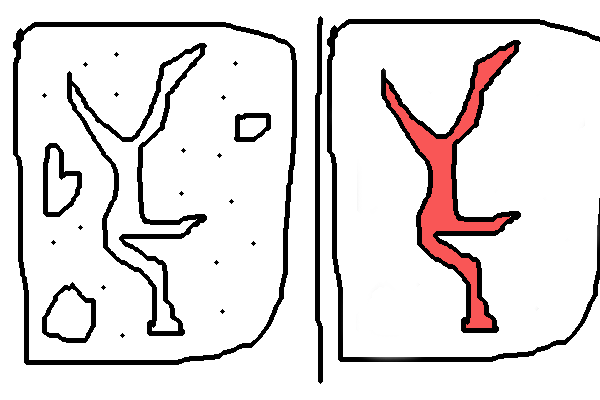
\includegraphics[height=5cm]{Images/example_enhancement.png}
  \label{fig:exemple_vesselness}
  \caption{exemple de filtre de rehaussement de vaisseaux}
\end{figure}

\section{Espace d'échelle}
\label{sec:EA:rehaussement:echelle}

La détection d'un réseau vasculaire dans sa totalité implique de détecter des vaisseaux de différentes tailles. En effet, les plus gros vaisseaux peuvent faire plusieurs dizaines de voxels de diamètres tandis que les vaisseaux les plus fins, atteignants les limites de la résolution des capteurs, peuvent  mesurer jusqu'à un voxel de diamètre. Il n'est pas envisageable de ré-écrire un algorithme pour chaque taille de vaisseaux, c'est pourquoi des cadres théoriques, appelés \emph{espace d'échelle} ont été formulés. Ces espaces d'échelles permettent d'établir un cadre uniforme pour sélectionner les structures d'une image à une échelle donnée. Trois espaces d'échelles sont courament associés au réhaussement de vasculaire dans la litterature : L'espace d'échelle gaussien, l'espace d'échelle granulométrique et l'espace d'échelle de flux orienté.

\subsection{Espace Gaussien}
\label{sec:EA:rehaussement:echelle:gaussien}

% what we want to say
% why gaussian ?
% - smoothing remove lower structures without introducing new ones
% - relation between sigma and sizes
% - relation to sigma and vessels radius
Lindenberg introduit la théorie de l'espace d'échelles gaussien dans \cite{lindeberg2013_scale}. Dans cette théorie, a l'échelle la plus basse, la totalité des structures sont présentes, et les détails les plus fins sont présents. Au fur et à mesure que l'échelle augmente, les détails sont lissés pour ne laisser que les maximas locaux correspondants aux formes les plus grandes. Ainsi, l'échelle minimale correspond à l'image initiale et l'échelle maximale correspond à une image uniforme. Il a été démontré que les noyaux gaussien étaient les seuls noyaux permettant de passer d'une échelle fine à une échelle grossière sans provoquer l'apparition de nouvelles structures. De plus, un mécanisme identique a été observé dans le fonctionnement du champ visuel.

\begin{figure}
  \centering
  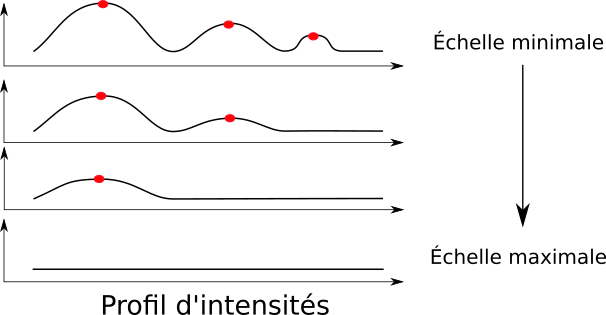
\includegraphics[height=5cm]{Images/gaussian_smoothing.png}
  \label{fig:gaussian_smoothing}
  \caption{Lissage gaussien, les structures de taille égales ou supérieures à $\sigma$ sont conservées alors que les structures de taille inférieures disparaissent}
\end{figure}

\begin{equation}
  gauss(x,y,\sigma_{x},\sigma_{y}) = \frac{1}{ \sigma\sqrt{2\pi} }exp(-\frac{x^2 + y^2 + z^2}{2(\sigma_{x}+ \sigma_{y}+ \sigma_{z}) })
\end{equation}

La sélection de l'échelle dans un espace gaussien se fait par le choix de l'écart-type $\sigma$ de la gaussienne. La plupart du temps on considère un espace d'échelle uniforme, $\sigma_x = \sigma_y = \sigma_z$. Il faut noter que pour un $\sigma$ donné, la taille des structures n'est pas supérieure ou égale à $\sigma$ mais plutôt supérieure ou égale à $\alpha\sigma$. En effet, en empruntant le formalisme des statistiques, l'interval de confiance, c'est-à-dire la couverture d'une distribution normale, correspond à $34.1\%$ pour $\sigma=1$, $68\%$ pour $\sigma=2$ et $99.7\%$ pour $\sigma=3$. Ainsi, pour $\sigma=1$ on détectera des objets de rayon $3\sigma$ et de diamètre $6\sigma$.  

\begin{figure}
  \centering
  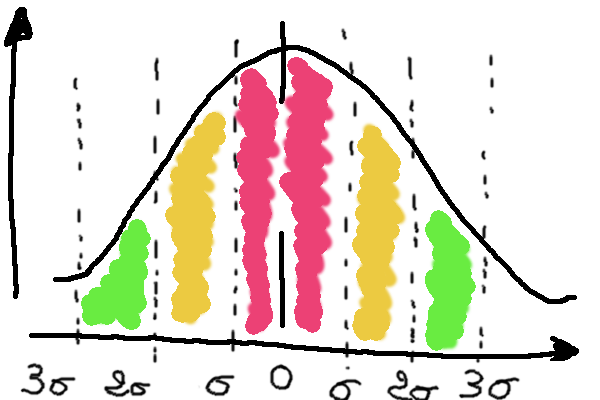
\includegraphics[height=5cm]{Images/normal_distribution_probability_coverage.png}
  \label{fig:normal_distribution_probability_coverage}
  \caption{couverture d'une distribution normale}
\end{figure}

L'espace gaussien se prète particulièrement bien à la modélisation des vaisseaux. En effet, la formulation de la gaussienne correspond bien à l'effet combiné des hypothèses de vaisseaux cylindriques et de la diminution d'intensité des vaisseaux au fur et à mesure que l'on s'éloigne de leur centre. En particulier pour un vaisseau parfait de diamètre $3\sigma$, les maximas locaux se situent le long de sa ligne centrale.

De plus, la gaussienne se prête très bien à une analyse locale de la géométrie basée sur la dérivation. Elle assure en effet les hypothèses de continuité du support de l'image et permet de combiner lissage et dérivation de l'image en une seule étape par dérivation du noyau gaussien.

Enfin, le lissage a l'avantage d'apporter une certaine robustesse au bruit et de compenser la perte locale de signal.

L'espace gaussien a toutefois des défauts. Le lissage de l'image implique nécessairement un étalement de toutes les structures qui peuvent par conséquent cacher des structures voisines de plus petites tailles. Ce phénomène est particulièrement observé lorsque plusieurs échelles sont étudiées. De même, deux structures adjacentes de même tailles peuvent fusionner, et ainsi créer une seule réponse, là où deux ojets existaient initialement.

\begin{figure}
  \centering
  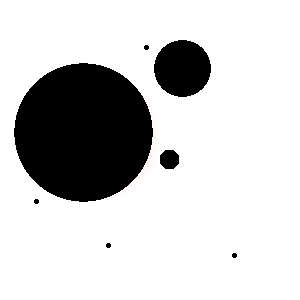
\includegraphics[height=3cm]{Images/gaussian_spilling_init.png}
  
\includegraphics[height=3cm]{Images/gaussian_spilling_g10.png}
  
\includegraphics[height=3cm]{Images/gaussian_spilling_g40.png}
  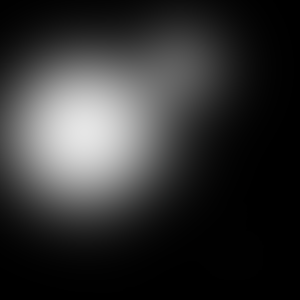
\includegraphics[height=3cm]{Images/gaussian_spilling_g100.png}
  \label{fig:scale_space_spilling}
  \caption{débordement du signal des structures larges sur les structures de plus petite tailles}
\end{figure}



\paragraph{Confirmation sur données réelles}

\todo{Expériences vérifiant en pratique la relation $3\sigma=diametre$}

\subsection{granulométrie}
\label{sec:EA:rehaussement:echelle:granulometrie}

La granulométrie est l'étude des tailles des particules d'un échantillon. En chimie, on utilise par exemple la technique du tamisage. Elle permet, grâce à un tamis et une grille dont on contrôle la taille du maillage, de ne conserver que des particules dont la taille est trop grosse pour passer à travers le tamis.

Un principe similaire est applicable en morphologie mathématique sur les images binaires et par extension en niveau de gris.

\subsubsection{Erosion et dilatation }

Deux opérations élémentaire, la dilatation et l'érosion, permettent de définir les opérations nécessaires pour définir un espace d'échelle morphologique. Les définitions qui vont suivre sont des opérations binaires relatives à des objets blancs sur fond noir.

\paragraph{Definitions}
% definition de Digital image processing, Gonzalez second edition, Mophology - p518
Soit deux ensembles définis dans $Z^3$ avec les composants $a=(a_1,a_2,a_3)$ et $b=(b_1,b_2,b_3)$.

La \emph{translation} de $A$ par $x = (x_1,x_2)$, noté $(A)_x$ est définie par :
% étrange cette formulation c|c non défini, idem pour x|x dans les autres.
\begin{equation}
  (A)_x = \{c|c = a+x, pour a \in A\}. 
\end{equation}

On définit la \emph{reflection} de B, dénoté $\widehat{B}$ par :

\begin{equation}
  (\widehat{B}) = \{x|x = -b, pour b \in B\}. 
\end{equation}

Le complémentaire de l'ensemble $A$ est défini par :

\begin{equation}
  (A^c) = \{x|x \not\in A\}. 
\end{equation}

La différence de deux ensemble $A$ et $B$, noté $A - B$, est défini par:

\begin{equation}
  (A-B) = \{x|x \in A, x\not\in \} = A \cap B^c.  
\end{equation}


\paragraph{dilatation}
En utilisant les propriétés précédentes, la dilatation s'exprime de la manière suivante :

\begin{equation}
 A \oplus B = {x|(\widehat{B}_x, \cap A \neq = \emptyset }
\end{equation}

La dilatation de $A$ par $B$ est l'ensemble de tous les déplacements de $\widehat{B}$ tel qu'il y ai au moins un pixel de recouvrement entre $A$ et $\widehat{B}$. Cette opération permet de faire grossir une structure en fonction de la forme de B.

\begin{figure}
  \centering
  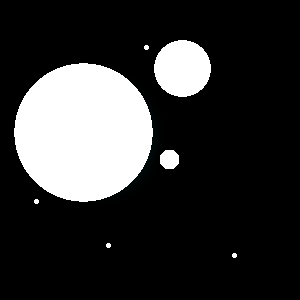
\includegraphics[height=3cm]{Images/morpho_init.png}
  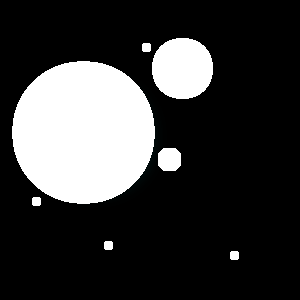
\includegraphics[height=3cm]{Images/morpho_dilate_k5.png}
  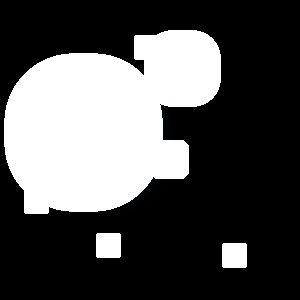
\includegraphics[height=3cm]{Images/morpho_dilate_k21.png}
  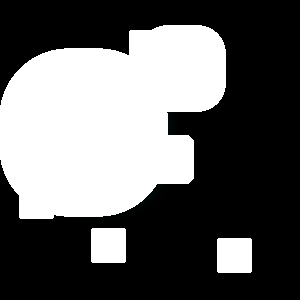
\includegraphics[height=3cm]{Images/morpho_dilate_k31.png}
  \label{fig:morpho_dilation}
  \caption{Exemple de dilatation}
\end{figure}

L'ensemble $B$ est courament appelé \emph{élement structurant}.

\paragraph{erosion}

L'opération oposée à la dilatation est l'érosion.

\begin{equation}
  A \ominus B = {x|(B)_x, \subseteq A}
\end{equation}

L'érosion de $A$ par $B$ est l'ensemble de tous les points $x$ tel que $B$ translaté de x est inclus dans $A$. 

\begin{figure}
  \centering
  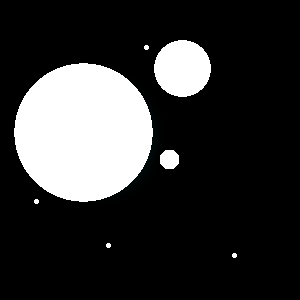
\includegraphics[height=3cm]{Images/morpho_init.png}
  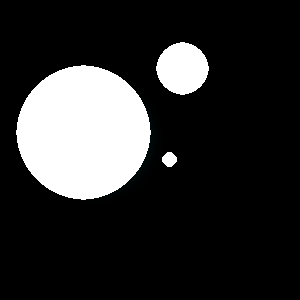
\includegraphics[height=3cm]{Images/morpho_erode_k5.png}
  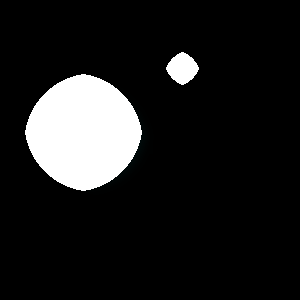
\includegraphics[height=3cm]{Images/morpho_erode_k21.png}
  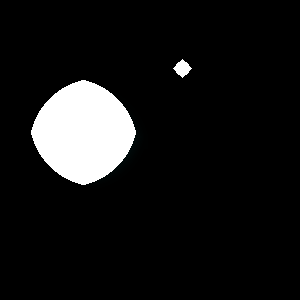
\includegraphics[height=3cm]{Images/morpho_erode_k31.png}
  \label{fig:morpho_erosion}
  \caption{Exemple d'érosion}
\end{figure}

\subsubsection{Fermeture et ouverture}

A partir des opérations d'érosion et de dilatation, on peut définir des opération composites, l'ouverture et la fermeture.

\paragraph{Fermeture}
L'ouverture est définie comme la dilatation de $A$ par $B$ suivi de l'érosion de $A$ par $B$.
\begin{equation}
 A \bullet B = (A \oplus B) \ominus B
\end{equation}

Cet opérateur est utilisé pour boucher les trous dont la surface est inférieure à la surface de l'élément structurant. L'érosion qui suit la dilatation permet d'assurer que la taille reste stable.

\begin{figure}
  \centering
  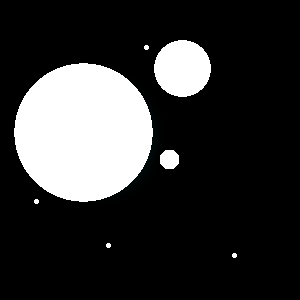
\includegraphics[height=3cm]{Images/morpho_init.png}
  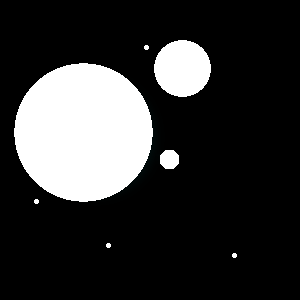
\includegraphics[height=3cm]{Images/morpho_close_k5.png}
  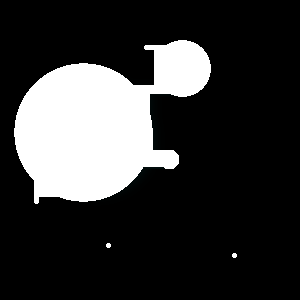
\includegraphics[height=3cm]{Images/morpho_close_k21.png}
  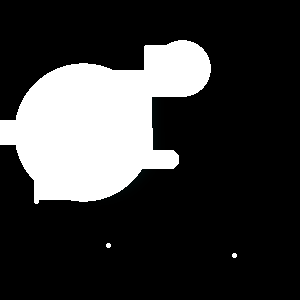
\includegraphics[height=3cm]{Images/morpho_close_k31.png}
  \label{fig:morpho_femerture}
  \caption{Exemple de fermeture}
\end{figure}

\paragraph{Ouverture}
L'ouverture est définie comme l'érosion de $A$ par $B$ suivi de la dilatation de $A$ par $B$.
\begin{equation}
 A \circ B = (A \ominus B) \oplus B
\end{equation}

\begin{figure}
  \centering
  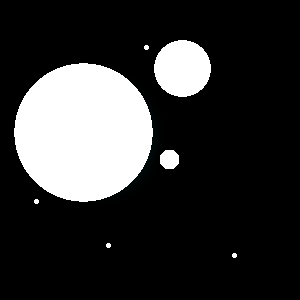
\includegraphics[height=3cm]{Images/morpho_init.png}
  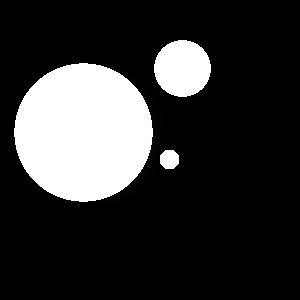
\includegraphics[height=3cm]{Images/morpho_open_k5.png}
  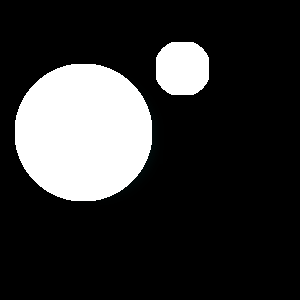
\includegraphics[height=3cm]{Images/morpho_open_k21.png}
  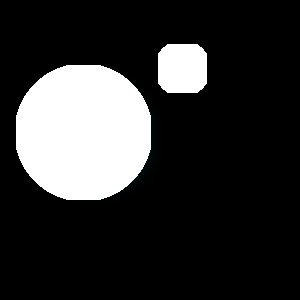
\includegraphics[height=3cm]{Images/morpho_open_k31.png}
  \label{fig:morpho_ouverture}
  \caption{Exemple d'ouverture}
\end{figure}

Cet opérateur est utilisé pour supprimer les structures de tailles inférieures à la surface de l'élément structurant. La dilatation qui suit l'érosion permet d'assurer que la taille des éléments restent stable.

L'ouverture permet de construire un espace d'échelle paramétré par la taille de l'élément structurant. Cet espace ne souffre pas d'une fusion parasite des structures adjacentes.

\subsection{Flux}
\label{sec:EA:rehaussement:echelle:flux}

Comme nous, l'avons vu dans la section , l'espace d'échelle gaussien peut provoquer des débordements de structures sur d'autres, plus petites. On peut limiter se problème en utilisant un cadre différent, celui de l'analyse des flux.

Si l'on considère un champ de vecteur $V$, par exemple un fluide, ou un champ de gradient pour une image, on défini le flux passant à travers la surface $S$ orienté par sa normale $\vec{n_s}$ comme l'intégrale de la somme du produit scalaire entre le vecteur de flux $\vec{v}$ et la normale à la surface $\vec{n}$.

\begin{equation}
flux_S = \int_{S}< \vec{v},\vec{n} > d\rho
\end{equation}

On peut appliquer le calcul de flux à la surface d'un objet fermé. En particulier, des structures en forme de disques ou de sphères ont été particulièrement utilisées pour l'analyse de vaisseaux sanguins. On peut en effet contrôler directement le diamètre d'une sphère pour détecter les objets de la taille voulue. Cette formulation de l'échelle diffère des méthodes précédentes, car les objets tubulaires ne sont détectés que pour une échelle donnée, là ou les deux autres techniques conservent les objets à l'échelle donnée et aux échelles supérieures. Elle a aussi l'avantage de limiter l'analyse du flux à la surface de la sphère et donc de produire une réponse qui ne déborde pas.

La précision du calcul de l'intégrale de flux dépend du nombre d'échantillonages effectués sur $S$. Plus celui-ci est grand, plus le calcul est coûteux. De plus, plus l'échelle sélectionnée est grande, et donc plus la surface de la sphère est grande, plus le nombre d'échantillonage requis est important.

Law propose une formulation élégante du calcul de flux dans le domaine de Fourier afin de réduire drastiquement le temps de calcul par rapport à l'implémentation naïve \cite{law2009_efficient_implementation}.

Pour y parvenir, law propose d'exprimer le calcul de flux sous la forme d'une convolution dans le domaine temporel. L'avantage de la convolution est double, on évite l'étape d'échantillonage sur la surface et la convolution s'exprime comme une multiplication dans le domaine de Fourier. On peut exprimer le calcul de flux en terme de volume et non plus en terme de surface grâce au théorème de la divergence qui établit une égalité entre le flux à la surface d'un objet et le flux à l'intérieur de son volume. Ainsi :

\begin{equation}
  flux_{\partial C} = \int_{\partial C}< \vec{v},\vec{n} > d\rho \equiv \int_{C }\Delta I d\nu
\end{equation}

Plus précisément :

\begin{equation}
  f_s(x,y,z) = \int_{R_s}\vec{v}(x+t,y+p, z+q) . \vec{n}_{(t,p,q)}dA
\end{equation}

avec $R_s$ une région sphérique de rayon $s$; $dA$ une surface infinitésimale sur la surface $\partial R_s$; $\vec{n}_{(t,p,q)}dA$ le vecteur normal à $dA$ à la position $(t,p,q)$; et $\vec{v}$ le gradient de l'image $I$. $\vec{v}$ est obtenu à partir de l'image $I$ lissée par un noyau Gaussien afin d'assurer la dérivabilité du signal de $I$. $\vec{v}=\nabla(g*I)$.

Qui est équivalent à :

\begin{align}
  f_s(x,y,z) & = \int_{R_s} \vec{div}( \vec{v}(x+t,y+p, z+q) ) dtdpdq \\
  & = \int_{\omega} d_s(t,p,q) [\vec{div}( \vec{v}(x+t,y+p, z+q) )] dtdpdq
\end{align}

où $\omega$ est le domaine entier de l'image et $d_s(t,p,q)$ correspond à la fonction porte sphérique définie par :

\begin{equation}
d_s(x,y,z) = [\sqrt{x^2 + y^2 + z^2} \leq s]
\end{equation}

Ainsi, $f_s(x,y,z)$ peut être exprimé sous forme de convolution :
\begin{align}
  f_s(x,y,z) & = \int_{\omega} d_s(t,p,q) [\vec{div}( \vec{v}(x+t,y+p, z+q) )] dtdpdq \\
             & = \int_{\omega} d_s(t,p,q) (\Delta(g*I(x+t,y+p, z+q)))] dtdpdq \\
             & = \int_{\omega} d_s(-t,-p,-q) (\Delta(g*I(x+t,y+p, z+q)))] dtdpdq \\
             & = d_s * \Delta g * I(x,y,z) \\
             & = I * h_s(x,y,z) \\
\end{align}

avec $*$ l'opérateur de convolution, $\Delta$ l'opérateur laplacien.

Et dans le domaine de Fourier:

\begin{align}
  FFT( I * h_s(x,y,z) ) &= FFT(I) . H_s(u,v,w) \\
                       &= FFT(I) . [ (j2 \pi)^2 ( (\frac{u}{N_x})^2 + (\frac{v}{N_y})^2 + (\frac{w}{N_z})^2 ) ] \\
                       & . [ exp( -( (\frac{u}{N_x})^2 + (\frac{v}{N_y})^2 + (\frac{w}{N_z})^2 ) 2(\pi\sigma)^2 ) ]
\end{align}

\begin{figure}
  \centering
  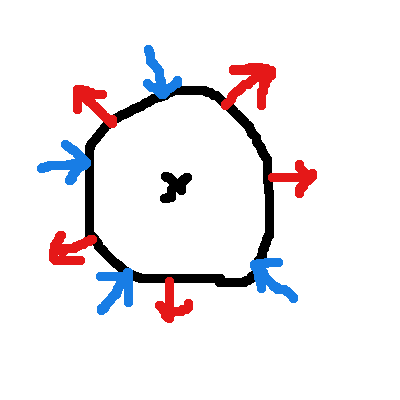
\includegraphics[height=6cm]{Images/flux.png}
  \label{fig:flux_sphere}
  \caption{flux sur la surface d'une sphère}
\end{figure}

\subsection{Multi-échelle}
\label{sec:EA:rehaussement:echelle:multiScale}

\todo{Voir si cette partie est à développer ici ou dans filtres, chapitre 4.}


\section{Familles de rehaussement}
\label{sec:EA:rehaussement:famille}

\begin{figure}
  \centering
  
\includegraphics[height=4cm]{Images/img_required.jpg}
  \label{fig:placeholder}
  \caption{placeholder}
\end{figure}

\subsection{Morphologie}
\label{sec:EA:rehaussement:morpho}

\subsection{Tensors}
\label{sec:EA:rehaussement:tensors}

% différents tensors, gradients,  

\subsection{Wavelets}
\label{sec:EA:rehaussement:wavelets}

% A voir comment articuler wavelets, noyaux gaussiens, etc.

\subsection{Hessienne}
\label{sec:EA:rehaussement:hessienne}

% Parler de la hessienne <-> co-occurence matrix et de leur explication géométrique. 
% parler des méthodes dont on ne traite pas par ailleur, Erdt, Li, etc.

\subsection{Diffusion}
\label{sec:EA:rehaussement:diffusion}

% VED
% HDCS

\section{Bilan et orientation des travaux}
\label{sec:EA:bilan}



